\newpage

\titleformat % design des titres des chapitres
{\chapter}
[display]
{\centering\normalfont\Large\scshape\bfseries}
{\rule[3pt]{0.15\linewidth}{3pt}\quad\chaptertitlename~\thechapter\quad \rule[3pt] {0.15\linewidth}{3pt}}
{0\baselineskip}%espace vertical entre chapitre et nom du chapitre
{\rule{\linewidth}{0.5pt}\break\Huge}
[\vspace{-0.5\baselineskip}\rule{\linewidth}{0.5pt}\vspace{0\baselineskip}]

\let\clearpage\relax% Stop LaTeX from going to a new page; and
\vspace*{5.5cm}%

\chapter{Réalisation du projet}
Dans ce chapitre, je vais présenter la réalisation du projet. D’abord je vais exposer
les interfaces de l’application, puis nous décrirons les différentes fonctionnalités de ces dernières.

\newpage

\section{Interface d'acceuil}

\begin{figure}[!h]
    \centering
    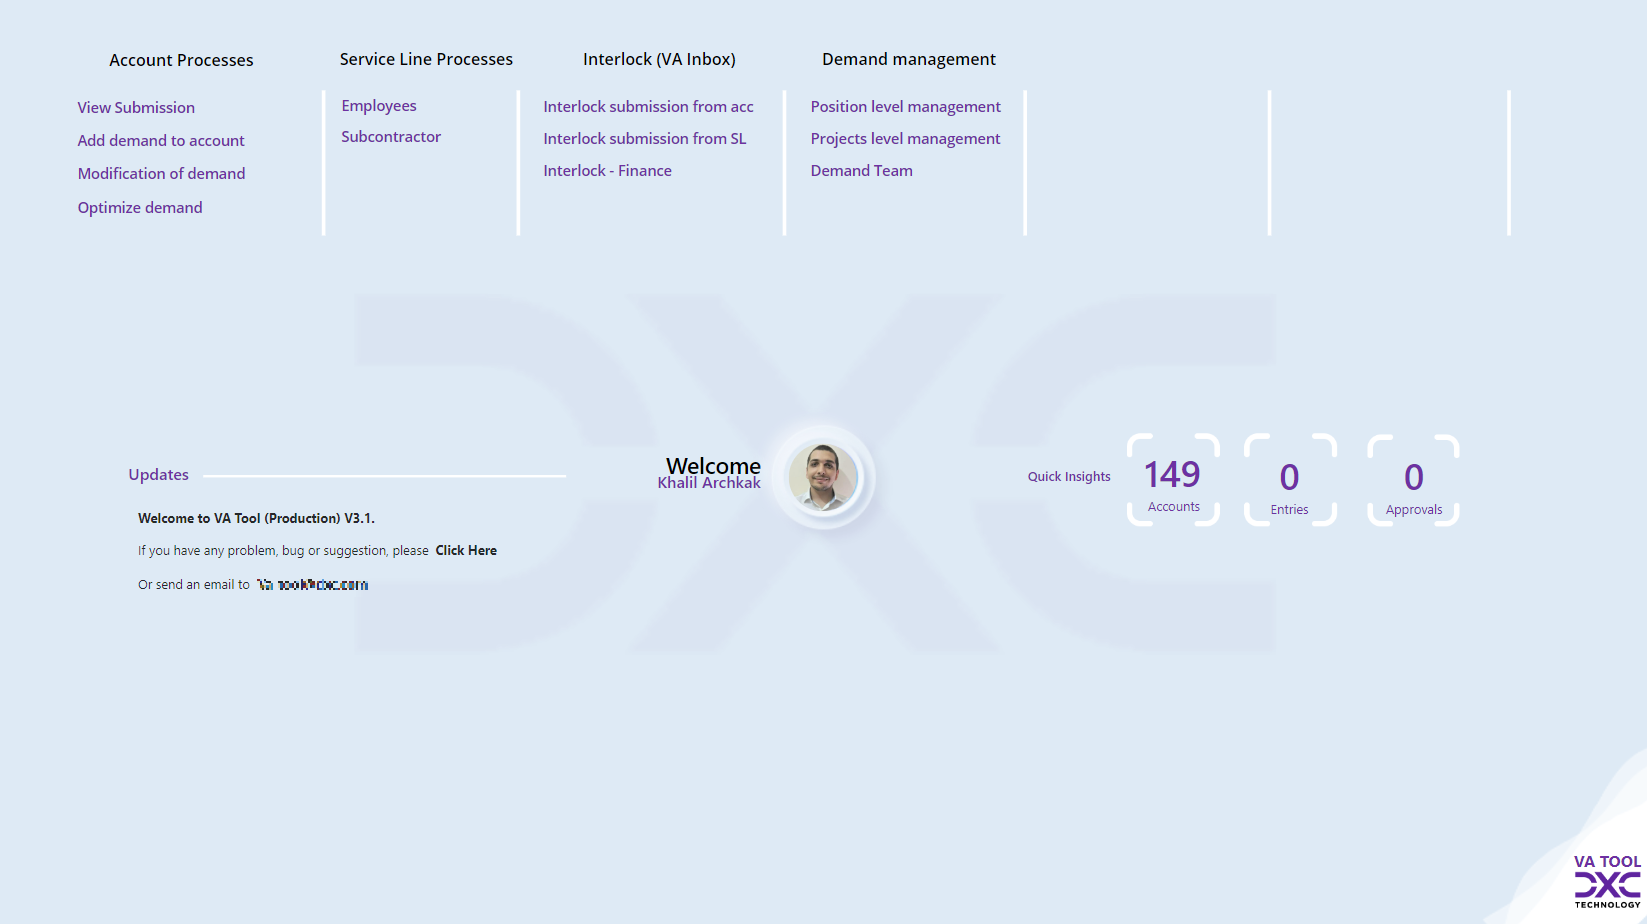
\includegraphics[scale=0.4,keepaspectratio]{Rapport de stage PFE chez DXC/figures/Home_Page.png}
    \caption{Interface d'accueil}
\end{figure}

La page d'accueil regroupe les différentes procédures possibles que propose l'application dans un menu verticale à savoir les procédures en relation avec les comptes, le service line, l'interlock de ces deux dernier mais aussi la gestion des demandes.
\\[0.3cm]
Elle contient aussi un aperçu rapide du nombre de compte affecté pour l'utilisateur, le nombre d'entré saisie par l'utilisateur mais aussi le nombre d'entré validé par ce dernier.
\\[0.3cm]
On peut aussi etre re-directionner vers une application d'aide ou bien envoyer un email en cas de problem a la mailbox de support. 

\newpage
\section{Compte - Ajout de masse salariale}
Pour l'ajout de masse salariale au niveau du compte 4 option se presente :

\begin{itemize}
    \item \textbf{Compte existant:} Le compte auxquelle on ajoute une demande existe déja en tant que client
    \item \textbf{New logo:}  Le compte auxquelle on souhaite ajouté une demande n'est pas encore un client
    \item \textbf{Roll-Off\Roll-on:} L'employé qu'on souhaite ajouter se trouve déja dans un autre projet et va changer ce dernier
    \item \textbf{PlaceHolder - add demand:} L'utilisateur souhaite créer une entré pour un future besoin
\end{itemize}

\subsection{Compte existant}

\begin{figure}[!h]
    \centering
    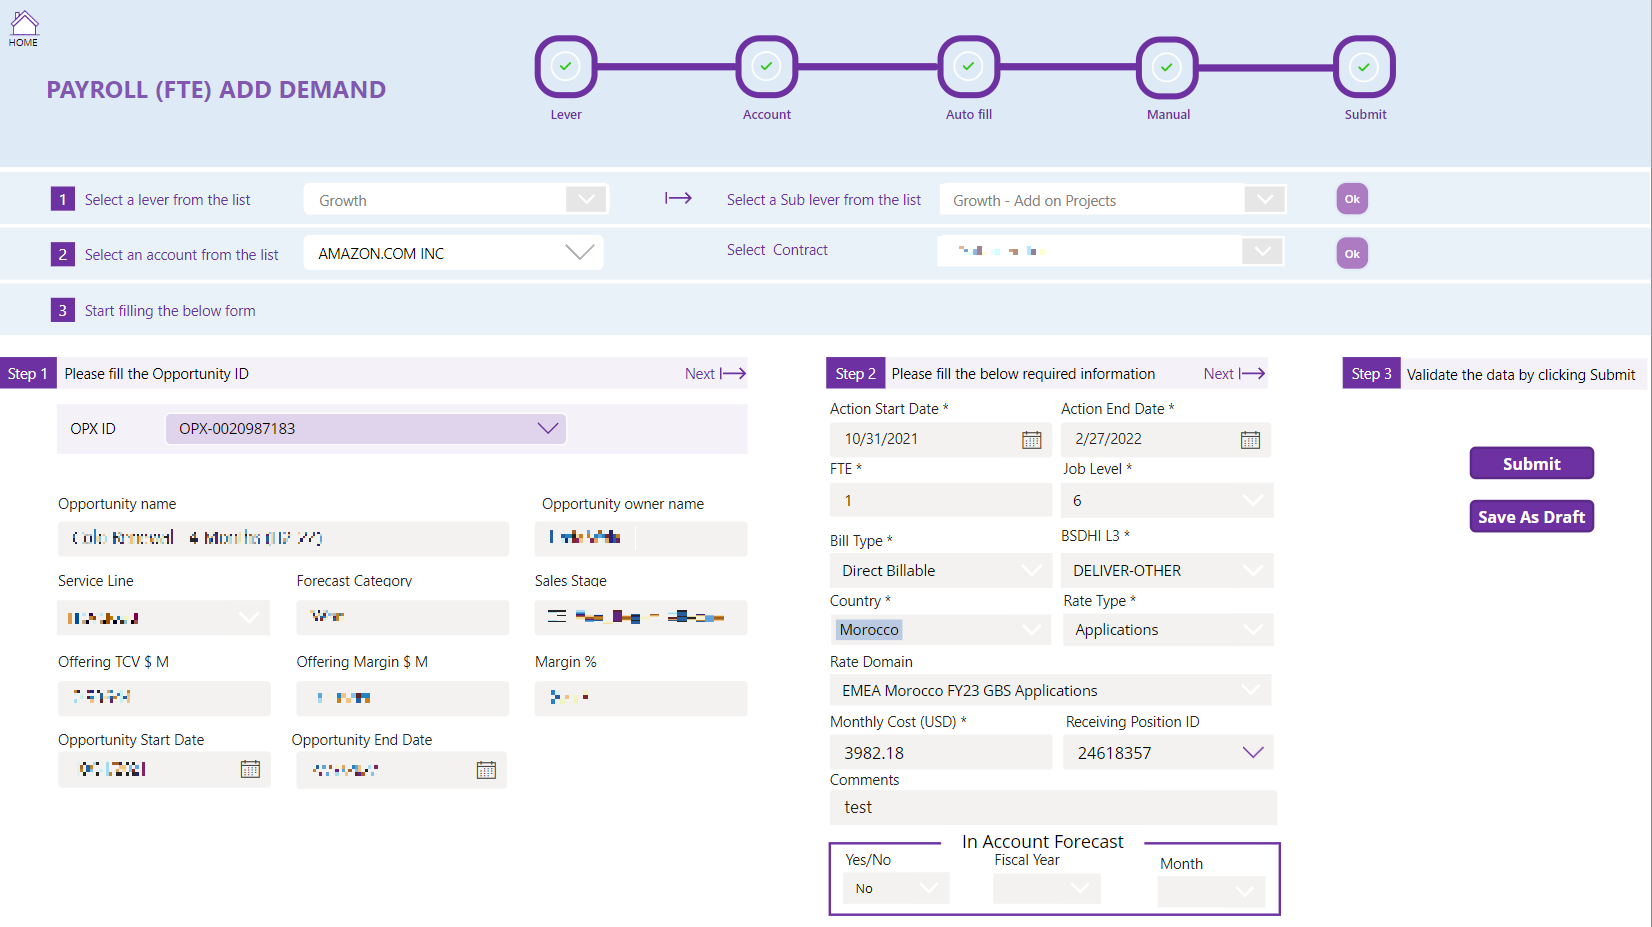
\includegraphics[scale=0.4,keepaspectratio]{Rapport de stage PFE chez DXC/figures/existin_account.png}
    \caption{Ajout de demande - Compte existant}
\end{figure}

L'utilisateur doit sélectionner le compte auxquelles il souhaite ajouter une demande, ensuite il doit saisir l'OPX-ID qui représente un identificateur pour une opportunité, ensuite toutes les informations de la première étape sont automatiquement remplies, puis l'utilisateur doit saisir les différentes informations de la deuxième étape en respectant les différentes contraintes. 
\\[0.3cm]
Deux options s’offrent à l'utilisateur pour saisir l’entrer il peut soit la soumettre directement ou bien l'enregistrer en tant que brouillon pour s'assurer des informations et la soumettre après.

\newpage
\subsection{New Logo}

\begin{figure}[!h]
    \centering
    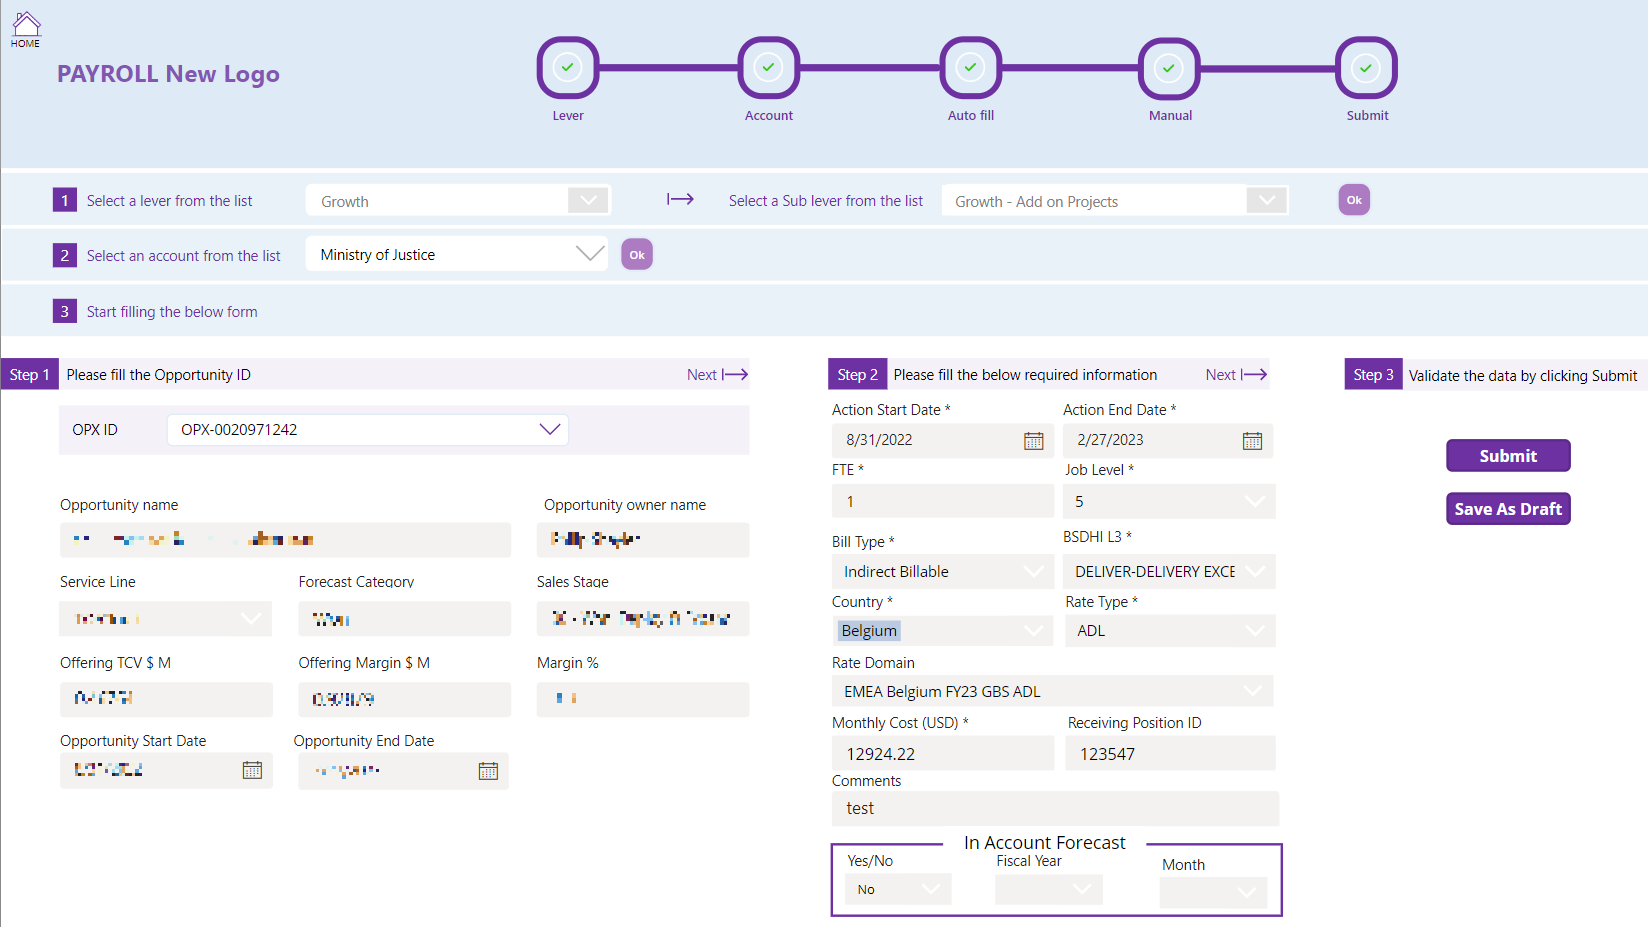
\includegraphics[scale=0.4,keepaspectratio]{Rapport de stage PFE chez DXC/figures/New_Logo.png}
    \caption{Ajout de demande - New Logo}
\end{figure}

Ce formulaire fonctionne de la meme facon que le precedent la seul difference est dans le choix du compte, dans ce dernier le choix du compte est fait a travers le contrat SalesForce car le compte n'est pas encore un client de DXC d'ou le nom de New Logo.

\subsection{Roll-Off / Roll-On}

\begin{figure}[H]
    \centering
    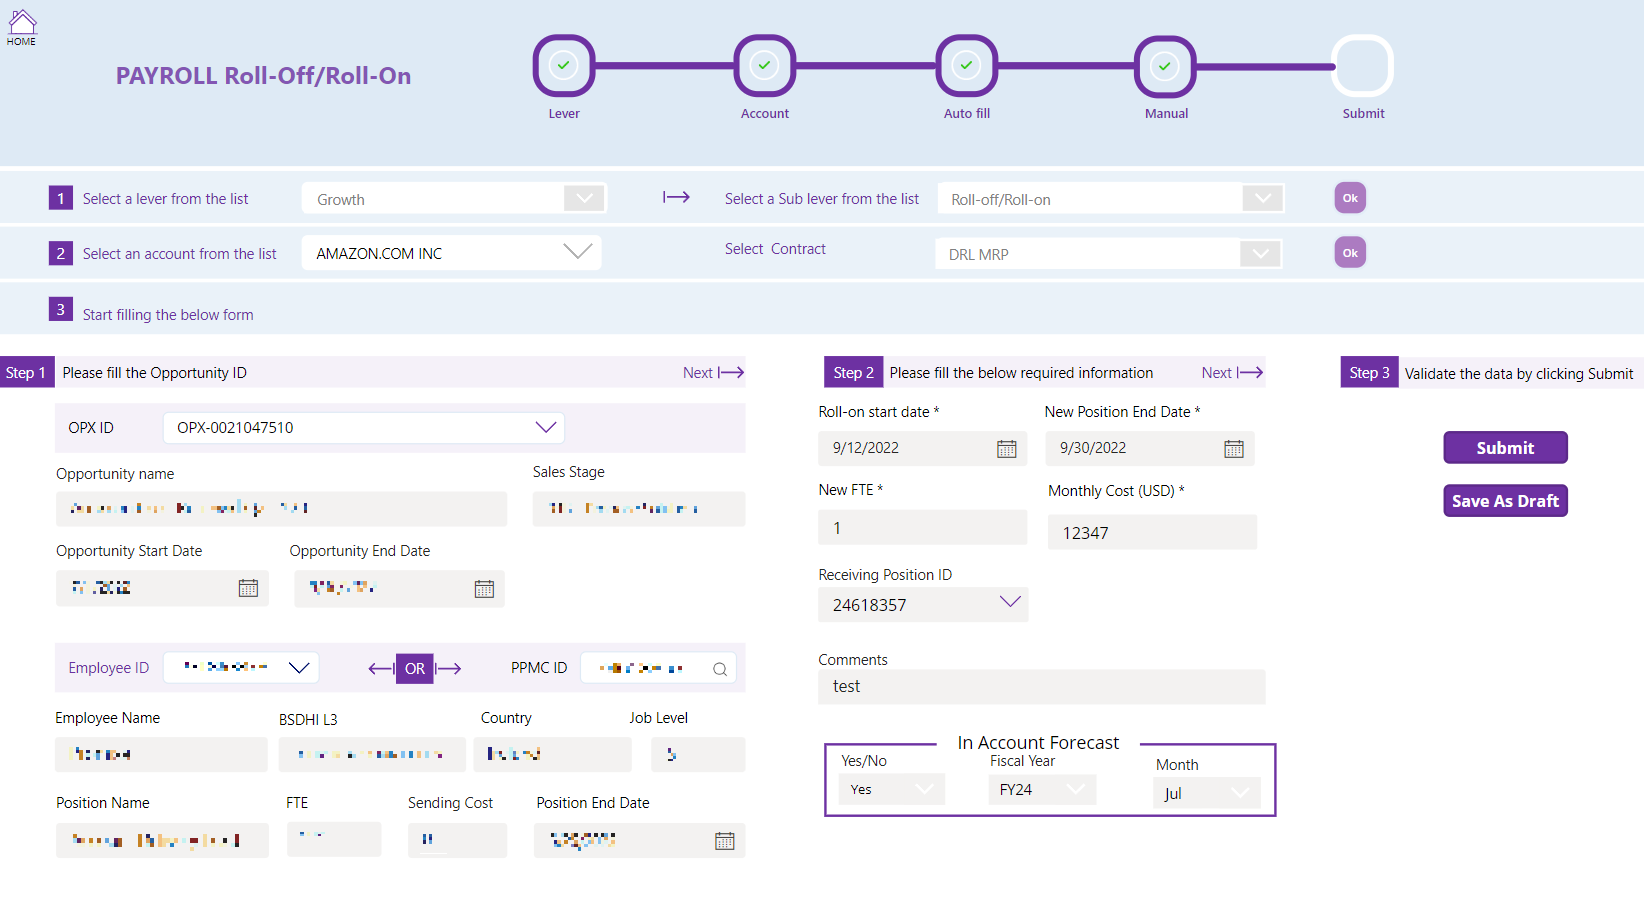
\includegraphics[scale=0.4,keepaspectratio]{Rapport de stage PFE chez DXC/figures/rolloff_rollon.png}
    \caption{Ajout de demande - Roll-Off / Roll-On}
\end{figure}

Pour le "Roll-Off/Roll-On", Un employé change de projet en restant avec le meme client.
\\
Dans la 1er etape l'utilisateur doit saisire l'OPX-ID mais aussi l'identificateur de l'employé qui vas faire la transition, ensuite il remplis les information necessaire dans la deuxieme étape tout en resepectant les differrentes contrainte, ensuite de la meme maniere il peut soit soumettre ou sauvegarder l'entré comme brouillon

\subsection{PlaceHolder - Add Demand}

\begin{figure}[H]
    \centering
    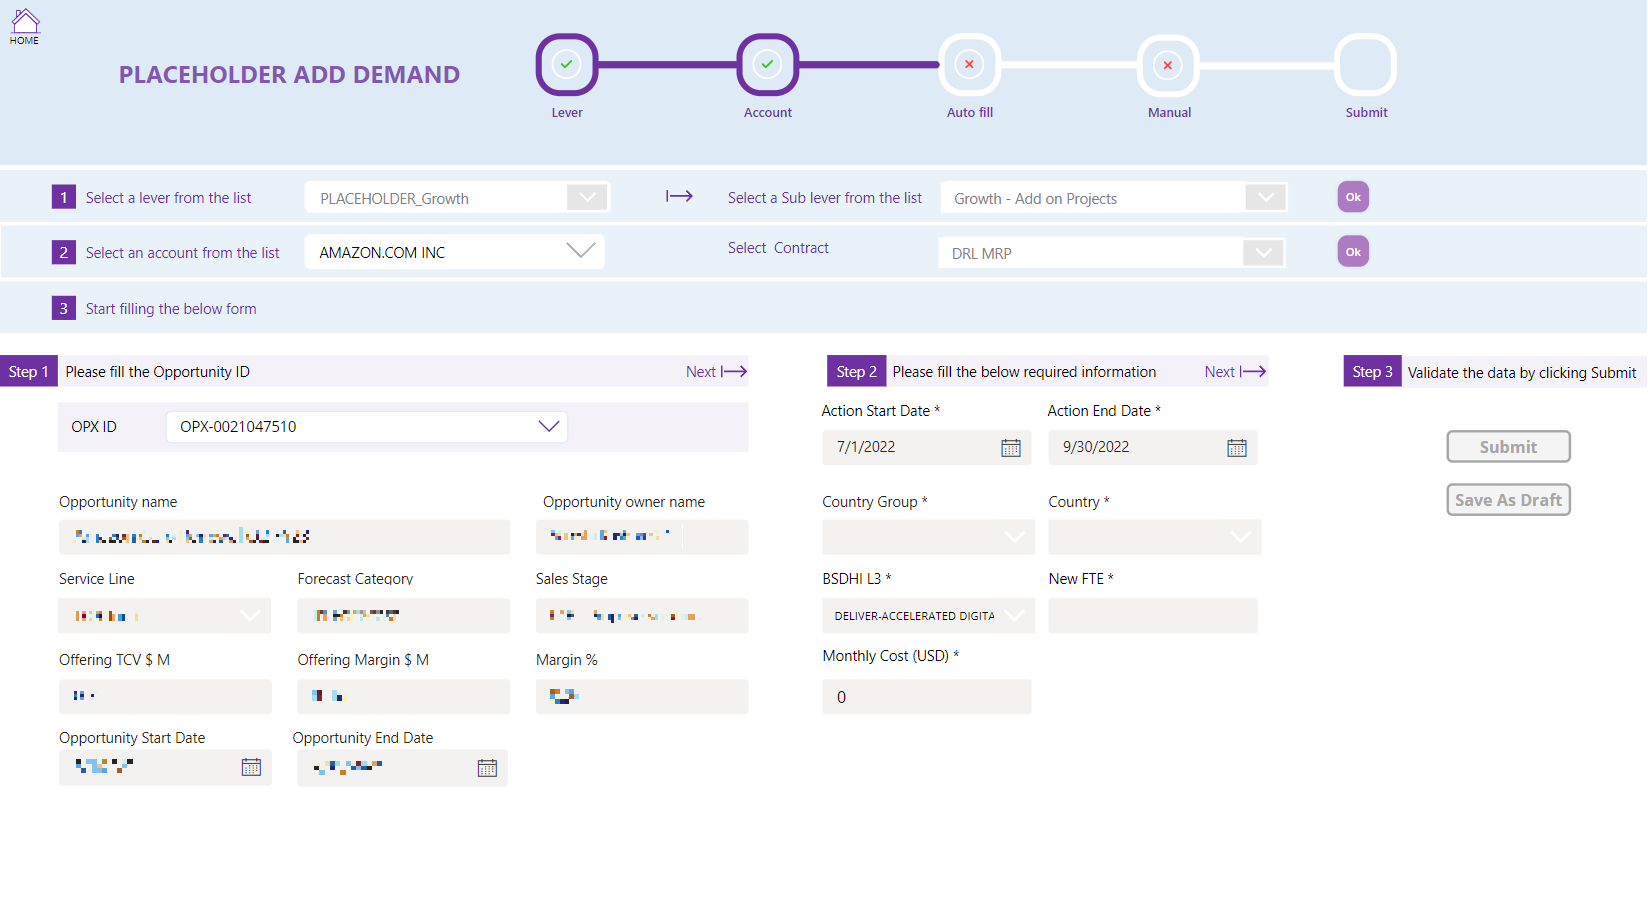
\includegraphics[scale=0.4,keepaspectratio]{Rapport de stage PFE chez DXC/figures/Placeholder_add_demand.png}
    \caption{Ajout de demande - Placeholder Add Demand}
\end{figure}

Pour les placeholders se sont des submission pour un future besoin, aprés avoir créer un placeholder ce dernier peut etre convertis ensuite en une entré VA dans la vue de submission, La soumission de cette entré se fait de la meme maniére que pour l'ajout de demande. 


\section{Compte - Modification de la masse salariale}

\subsection{Modification de la masse salariale}
\begin{figure}[H]
    \centering
    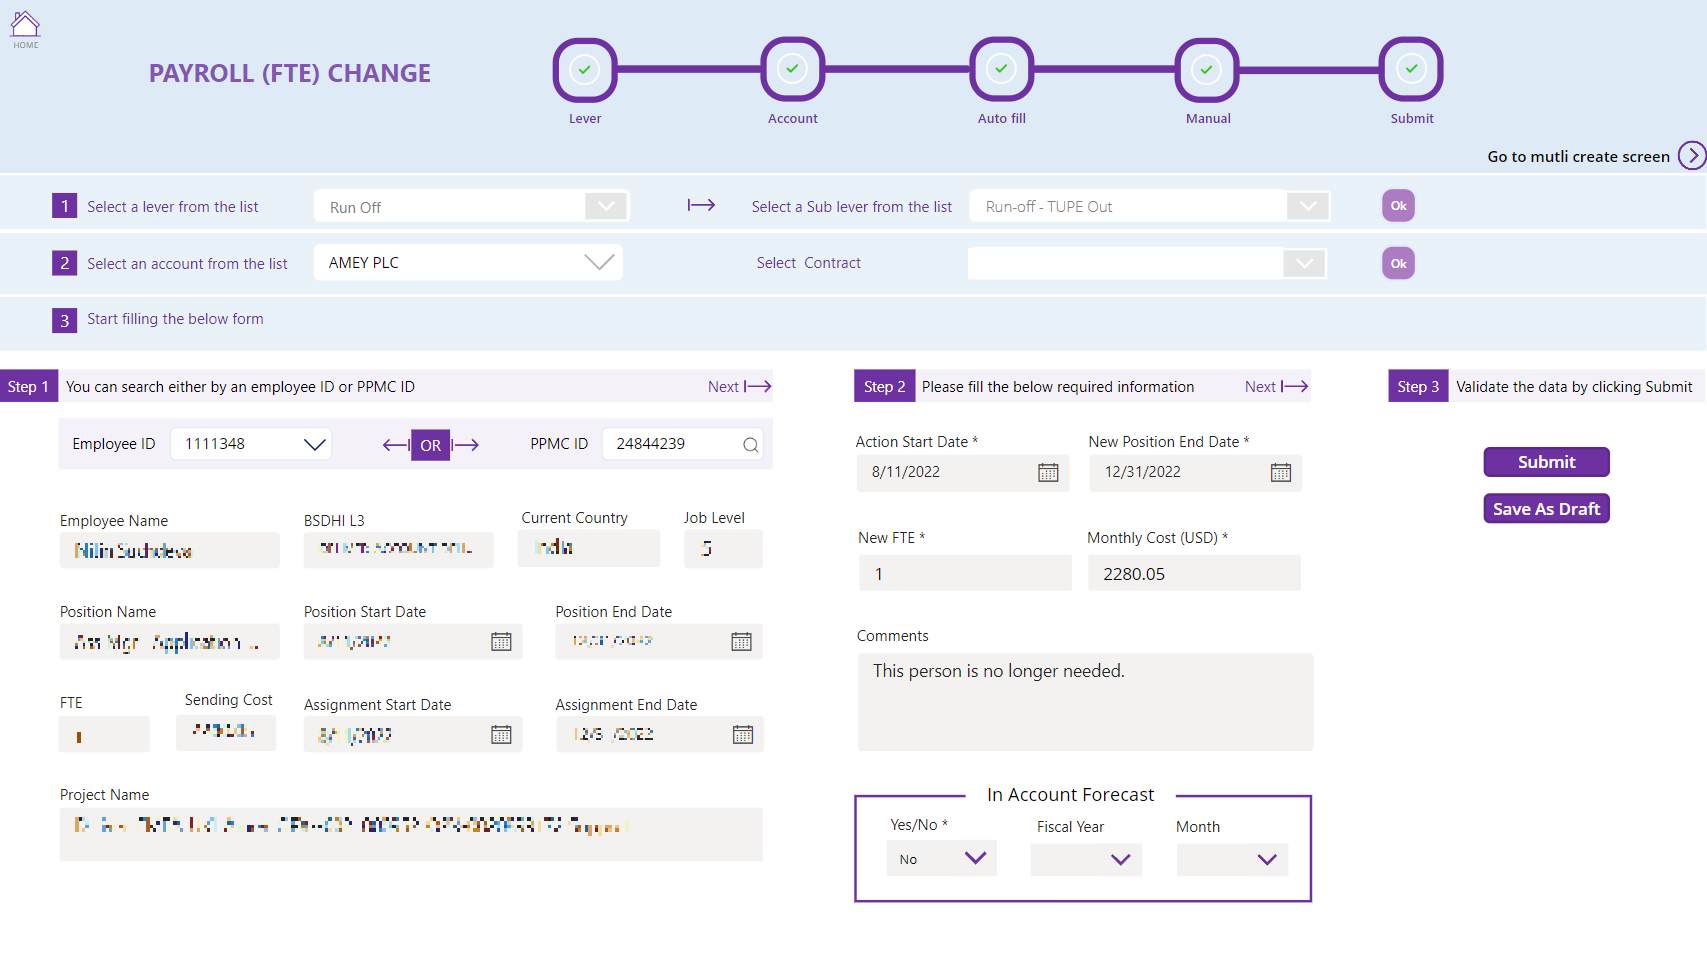
\includegraphics[scale=0.4,keepaspectratio]{Rapport de stage PFE chez DXC/figures/modification_of_demand.png}
    \caption{Compte - Modification de la masse salariale}
\end{figure}

La modification de demande peut etre soit un "Run-Off" c'est a dire une personne qui quitte son poste ou bien une "extension" ou la personne voit sont contract étendue, le processus est a peu prés le meme, l'utilisateur choisi l'employé ensuite remplie les information necessaire de la deuxieme étape et par la suite saisi son entrés.

\newpage

Dans la plupart des cas l'utilisateur a plusieurs entré a saisire dans ces deux lever, choisir a chaque fois un employé remplire les meme information puis sasire l'entré peut devenir redondant c'est pour cela qu'un module de multi-creation a été fait :

\begin{figure}[H]
    \centering
    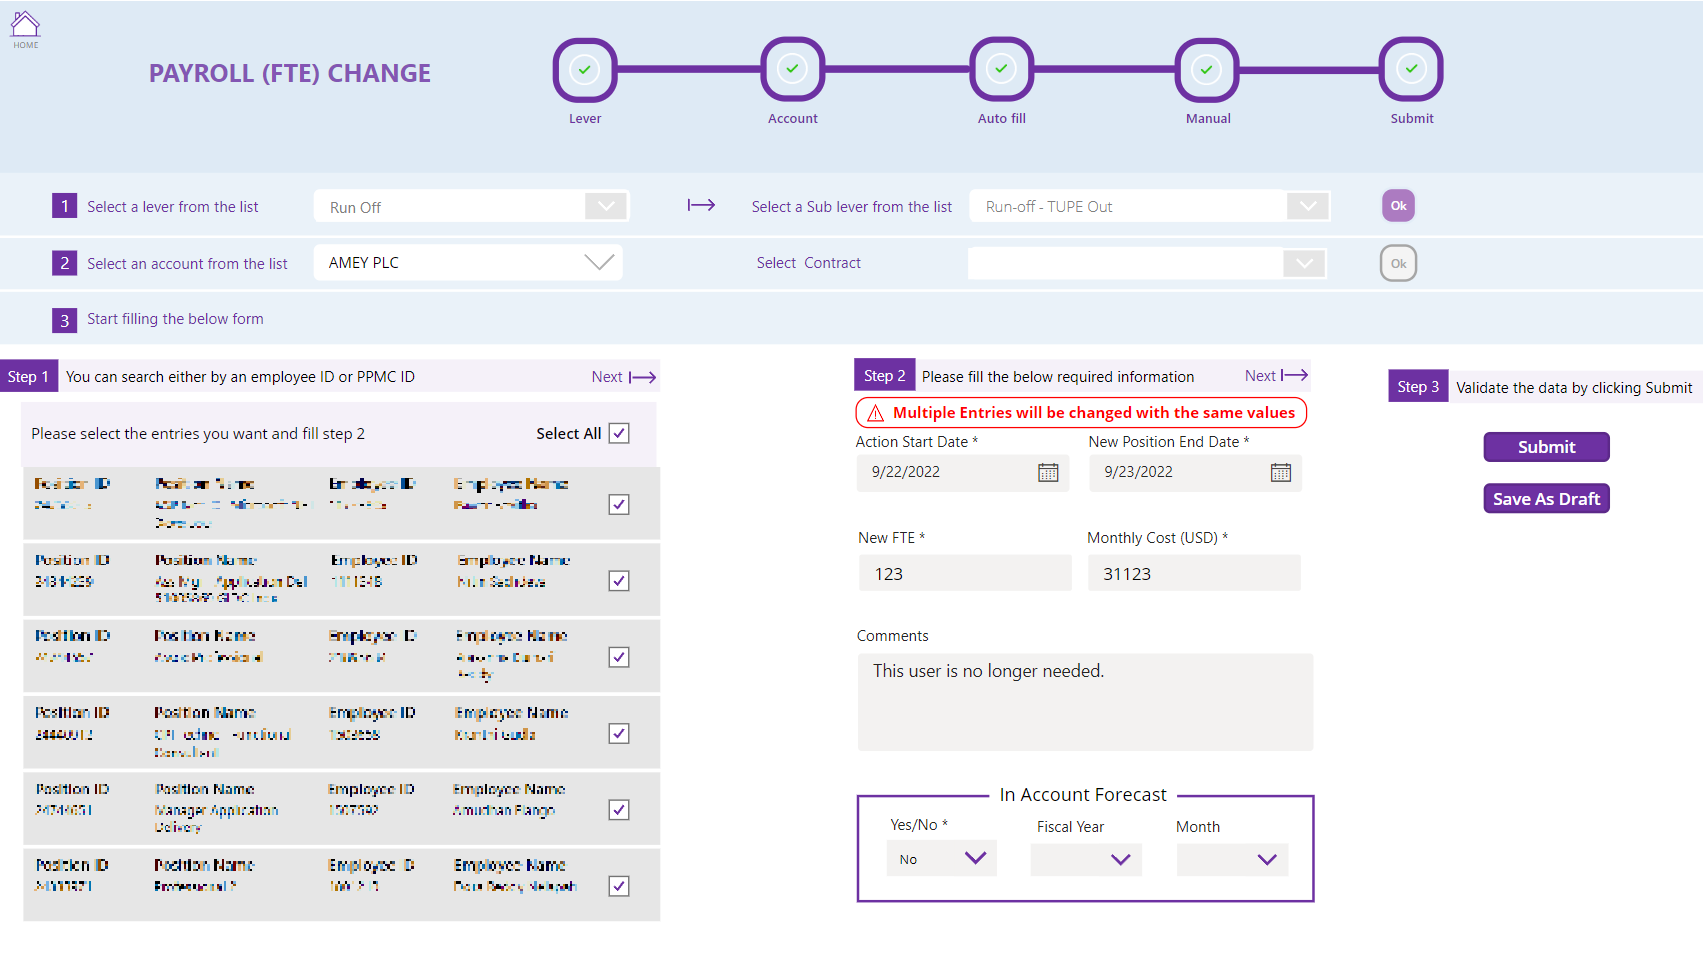
\includegraphics[scale=0.4,keepaspectratio]{Rapport de stage PFE chez DXC/figures/multi_modification_of_demand.png}
    \caption{Compte - Modification de la masse salariale en grand nombre}
\end{figure}

La seul difference entre les deux module et le fait que l'utilisateur peut choisir plusieurs utilisateur a la fois ces dernier auront les meme information et le systeme va créer automatiquement une entré par utilisateur selectionné.

\newpage

\subsection{Placeholder Modification de la masse salariale}

De la meme maniere que le placeholder pour l'ajout de demande, le placeholder de modification de demande permet a l'utilisateur de créer des entrée pour des future besoin :

\begin{figure}[H]
    \centering
    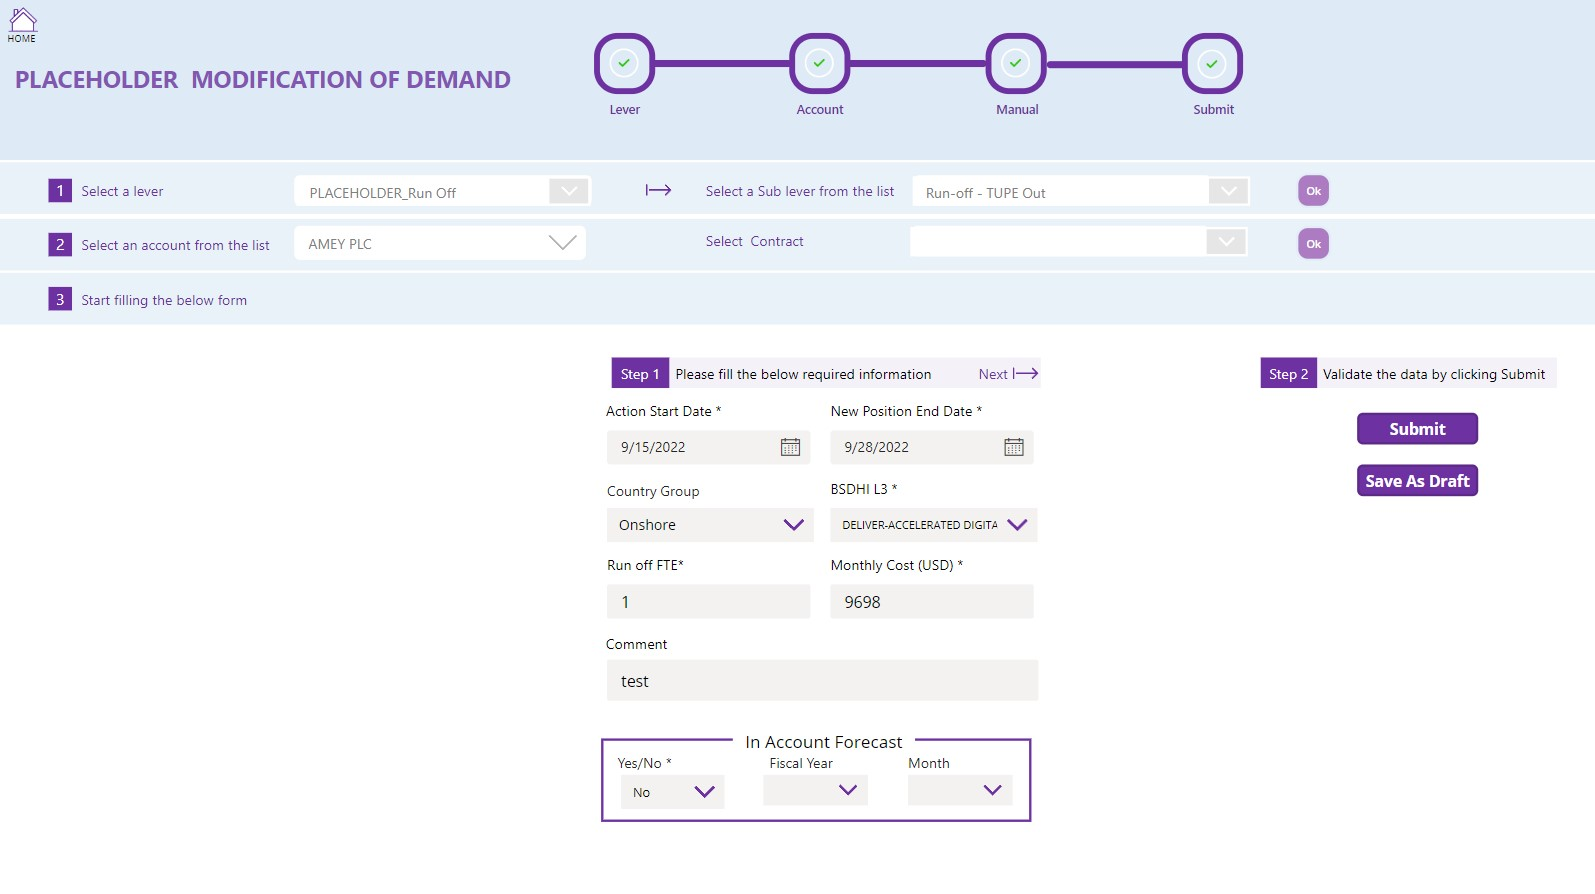
\includegraphics[scale=0.4,keepaspectratio]{Rapport de stage PFE chez DXC/figures/placeholder_modification_of_demand.jpg}
    \caption{Placeholder - Modification de la masse salariale}
\end{figure}

Ce dernier ne contient pas tout les informations necessaire pour une entrée run-off mais peut etre ensuite convertit en une entrée VA avec tout les information necessaire.

\newpage
\section{Compte - Consultation des soumissions}

Le module de consultation des soumissions est composé de plusieurs filtre qui vont permettre a l'utilisateur de facilement trouver son entrée 

\begin{figure}[H]
    \centering
    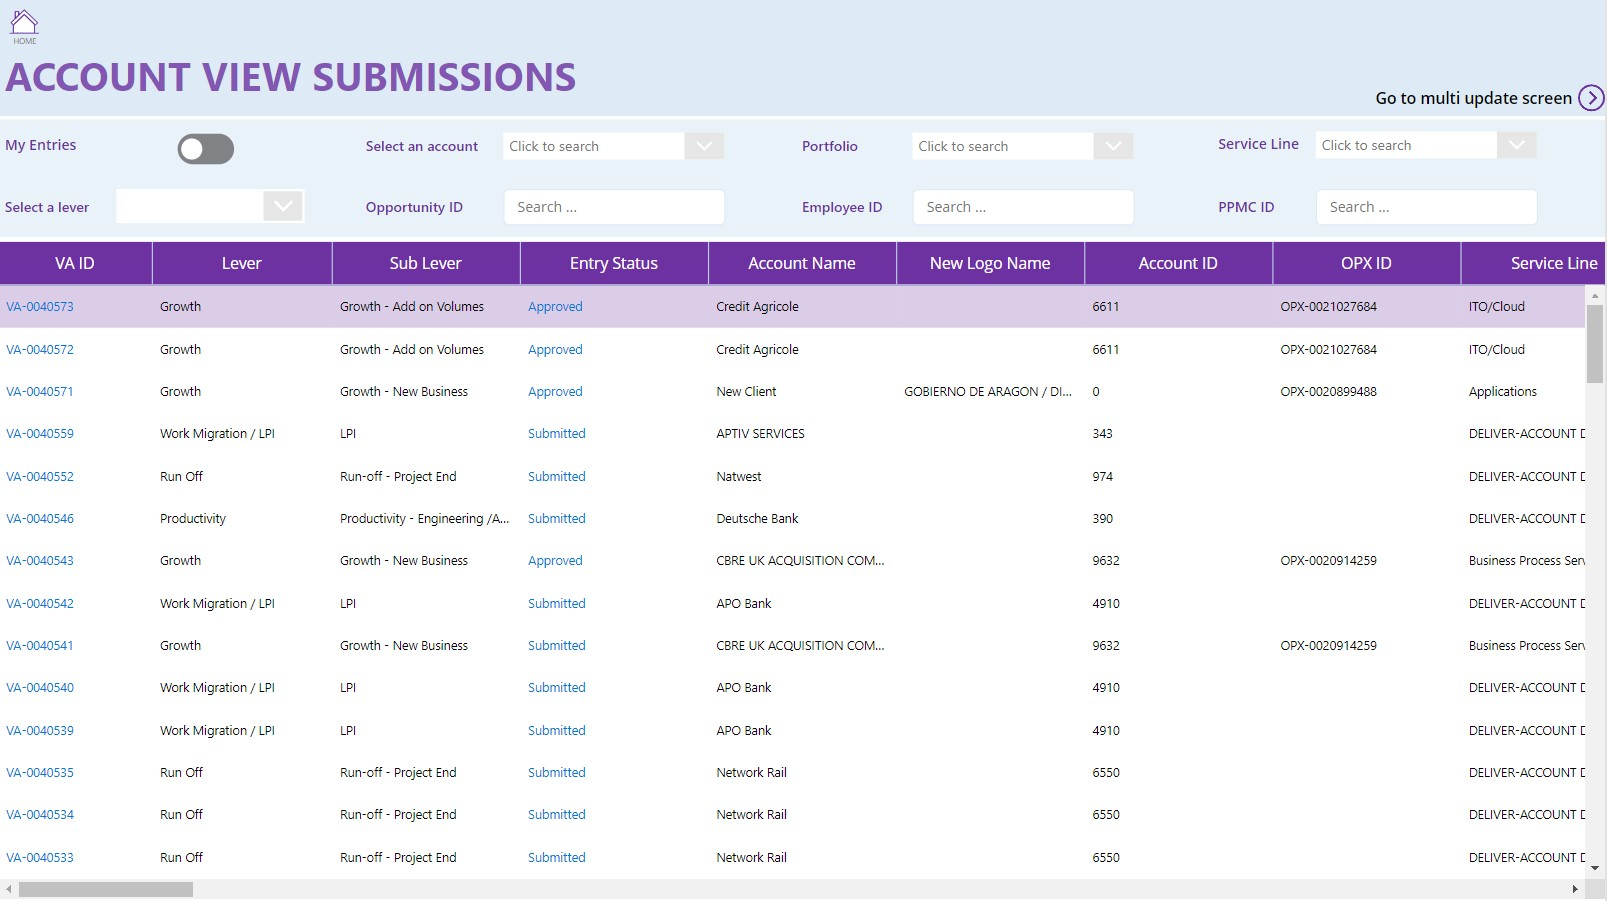
\includegraphics[scale=0.4,keepaspectratio]{Rapport de stage PFE chez DXC/figures/view_submission.jpg}
    \caption{Compte - Consultation des soumissions}
\end{figure}

En plus de cela en cliquant sur une entré nous avons un menu latéral qui vas nous permettre de modifier les information de l'entrer puise enregistre, ou bien 
dupliquer l'entrée mais aussi créer une entrée DCT a partir de cette derniere :

\begin{figure}[H]
    \centering
    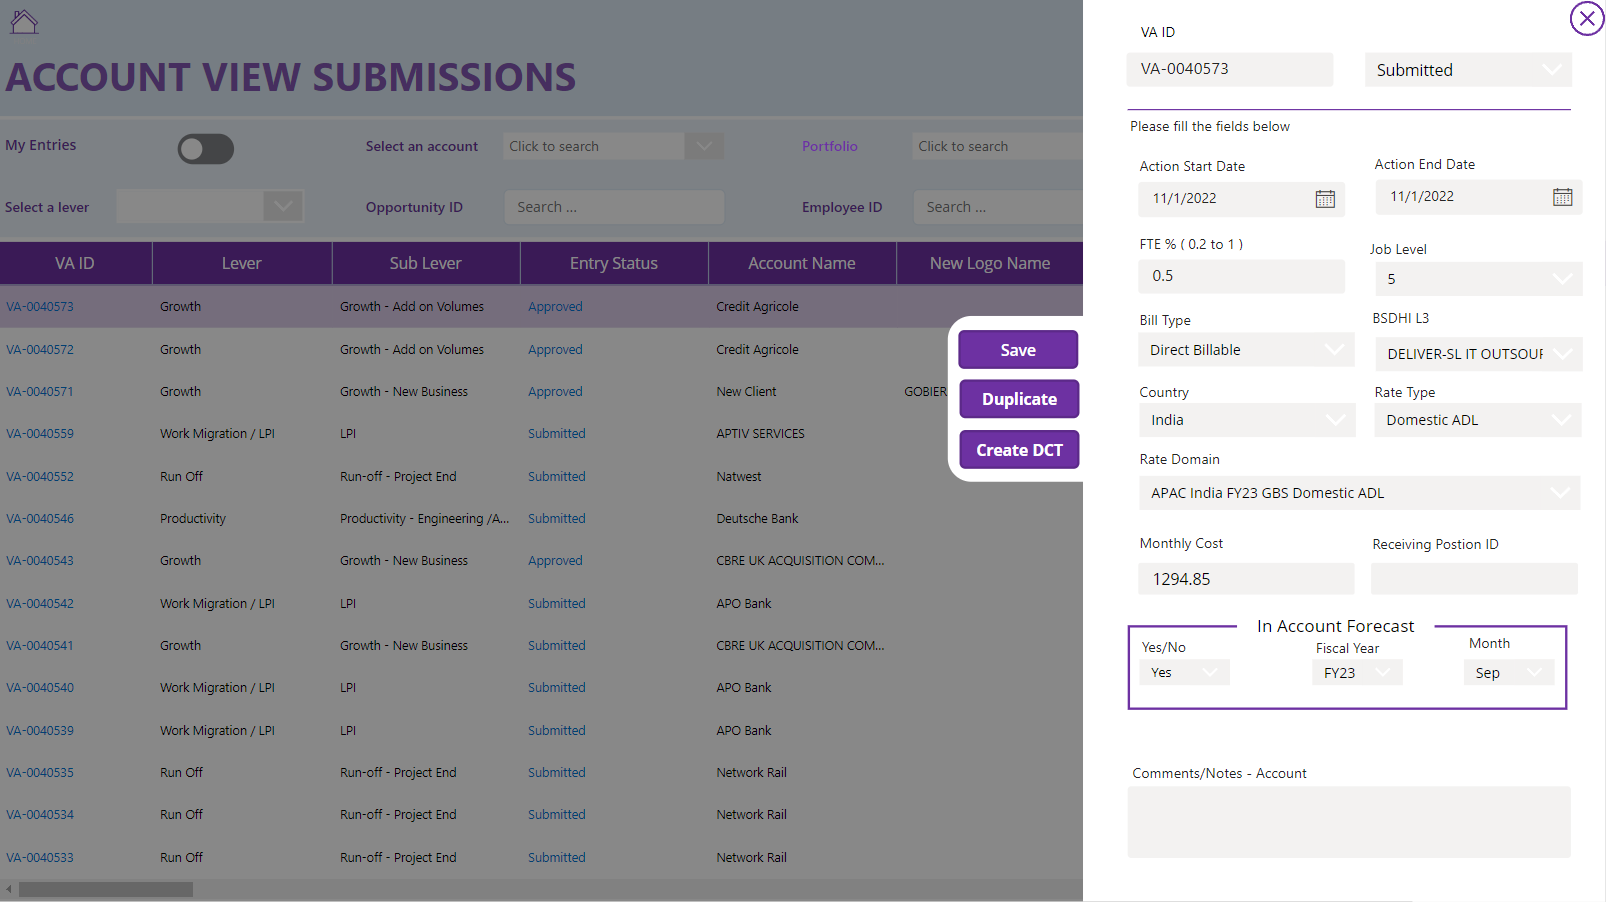
\includegraphics[scale=0.4,keepaspectratio]{Rapport de stage PFE chez DXC/figures/account_view_side_menu.png}
    \caption{Compte - Consultation des soumissions - Menu latéral}
\end{figure}

\section{DCT Position Level Management}

\subsection{DCT Position Level Management - Creation de demande}

DCT est l'acronyme de Demand creation template, Pour ce screen l'utilisateur peut créer une demande de croissance : 

\begin{figure}[H]
    \centering
    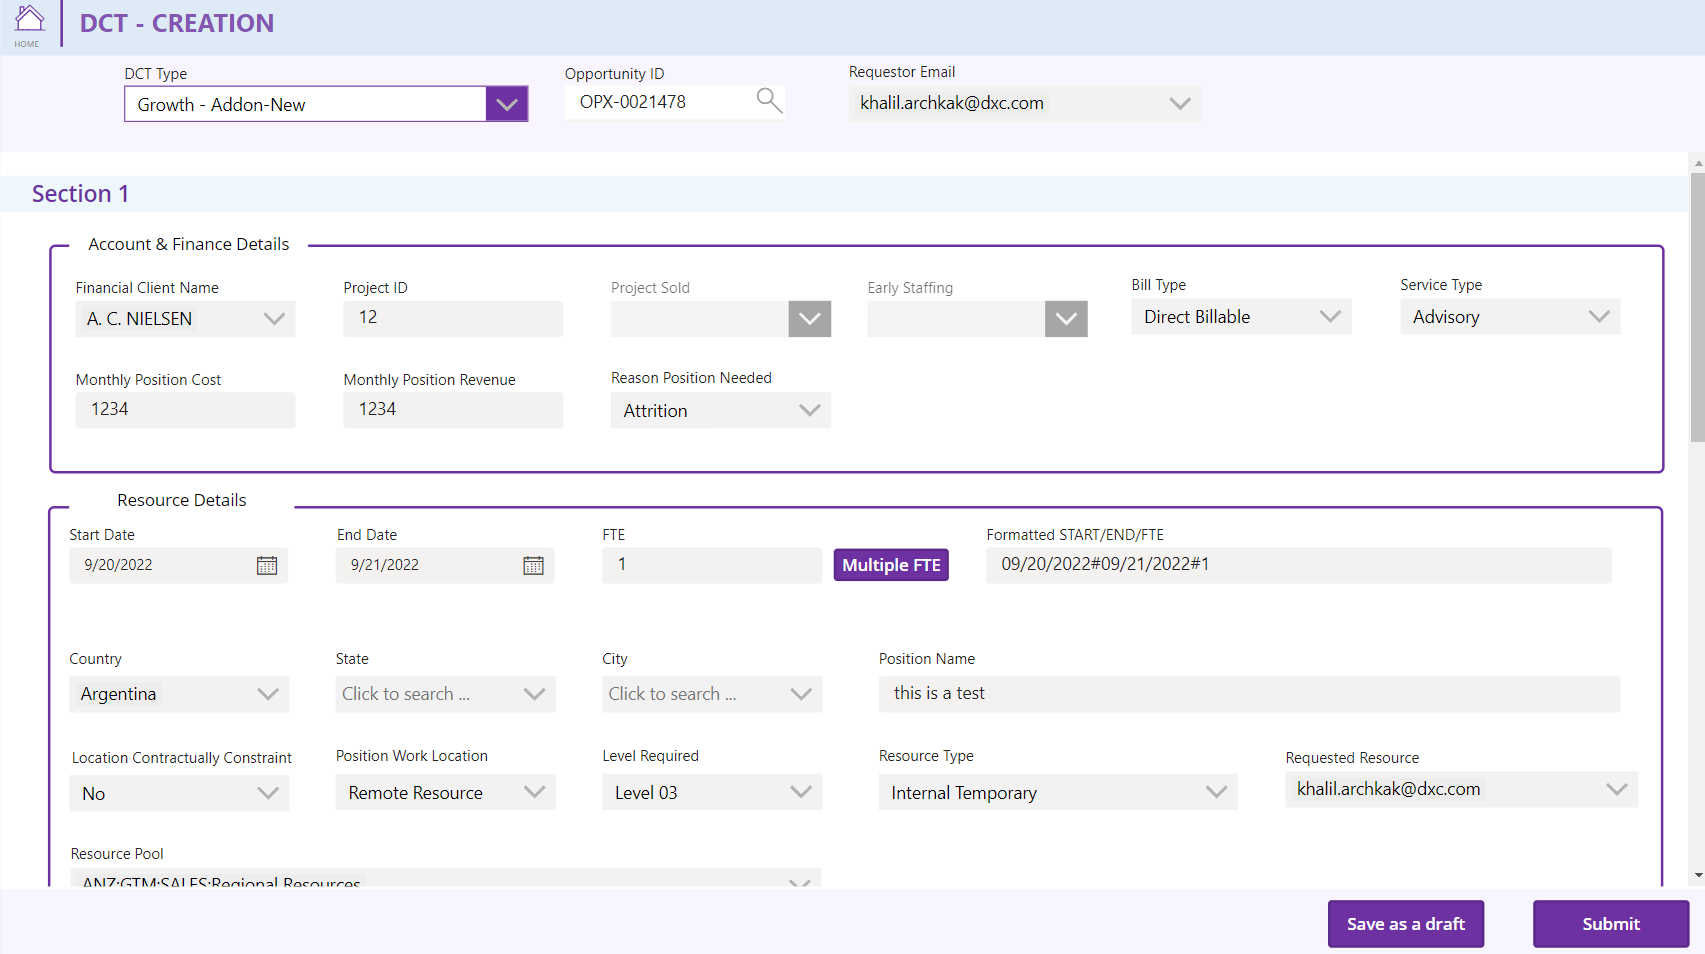
\includegraphics[scale=0.4,keepaspectratio]{Rapport de stage PFE chez DXC/figures/DCT_Create.png}
    \caption{DCT Position Level Management - Creation de demande }
\end{figure}

Le formulaire est composée de plusieurs champ a remplire avec differentes information, la plupart sont automatiquement remplie a travers les information precedente, ces derniers sont aussi vérifier pour n'avoir que des donnée valide.

\subsection{DCT Position Level Management - Mise a jour de la demande}

Ce screen permet de saisire une modification au niveau d'un DCT, il a le meme principe que le precedent : 

\begin{figure}[H]
    \centering
    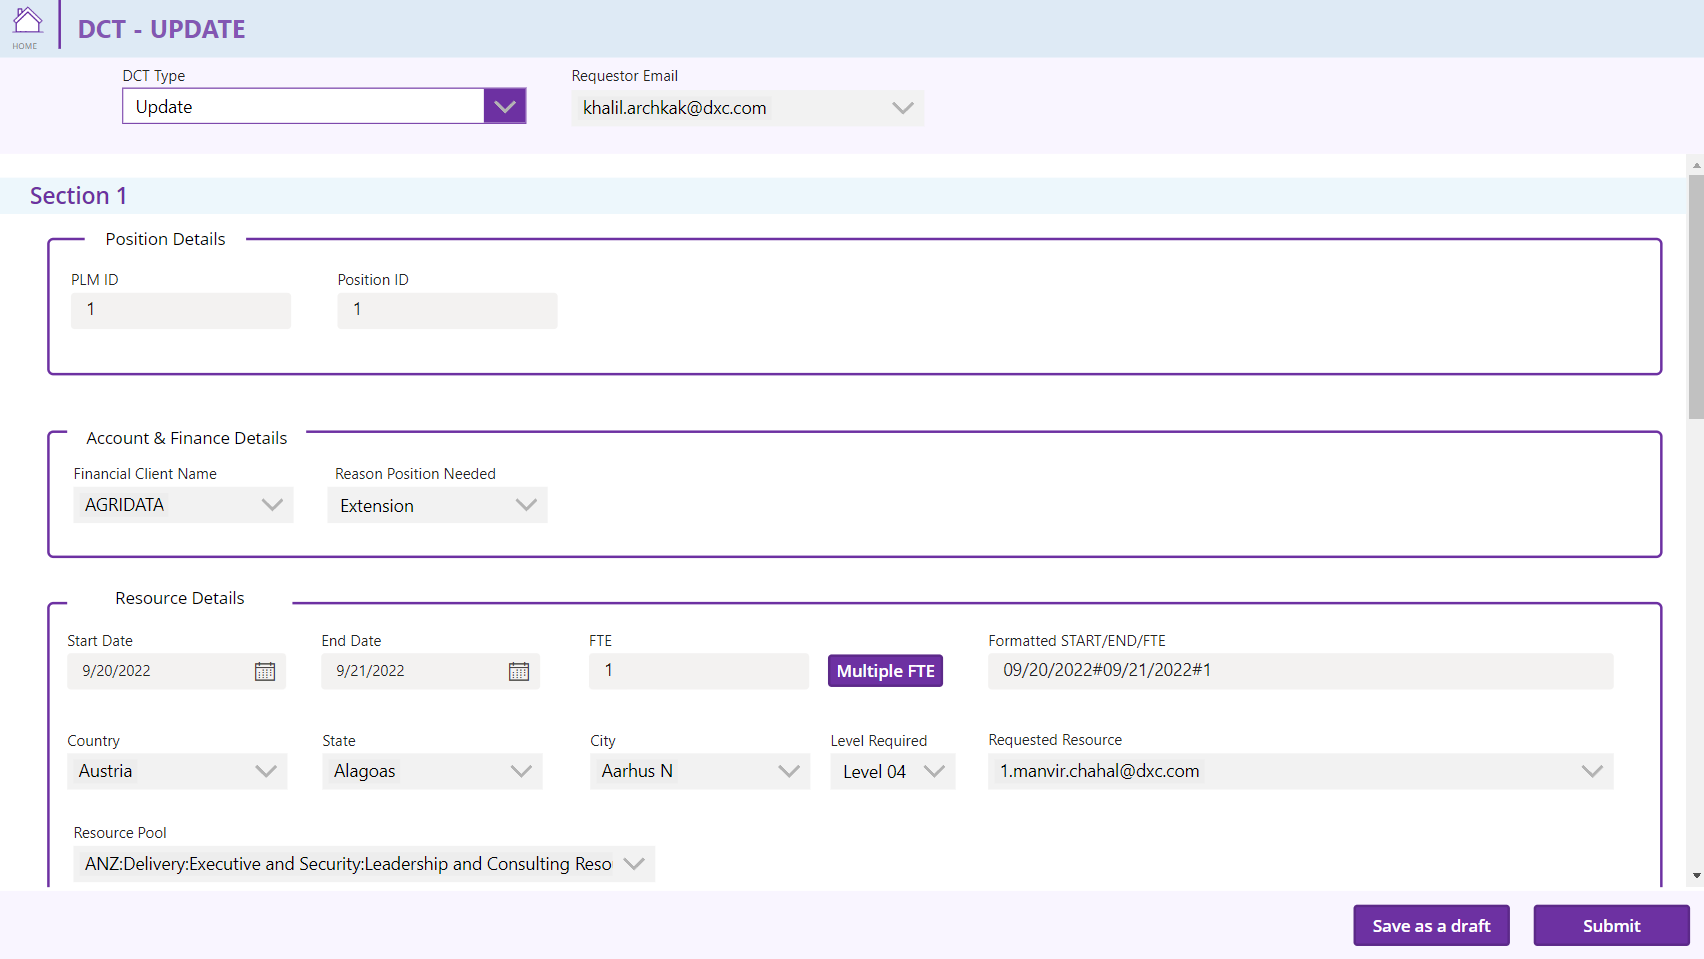
\includegraphics[scale=0.4,keepaspectratio]{Rapport de stage PFE chez DXC/figures/DCT_Update.png}
    \caption{DCT Position Level Management - Mise a jour de la demande}
\end{figure}

\subsection{DCT Position Level Management - Consultation des soumissions}

Aprés avoir saisit l'entrée l'utilisateur est envoyé vers le screen de consultation des soumissions:


\begin{figure}[H]
    \centering
    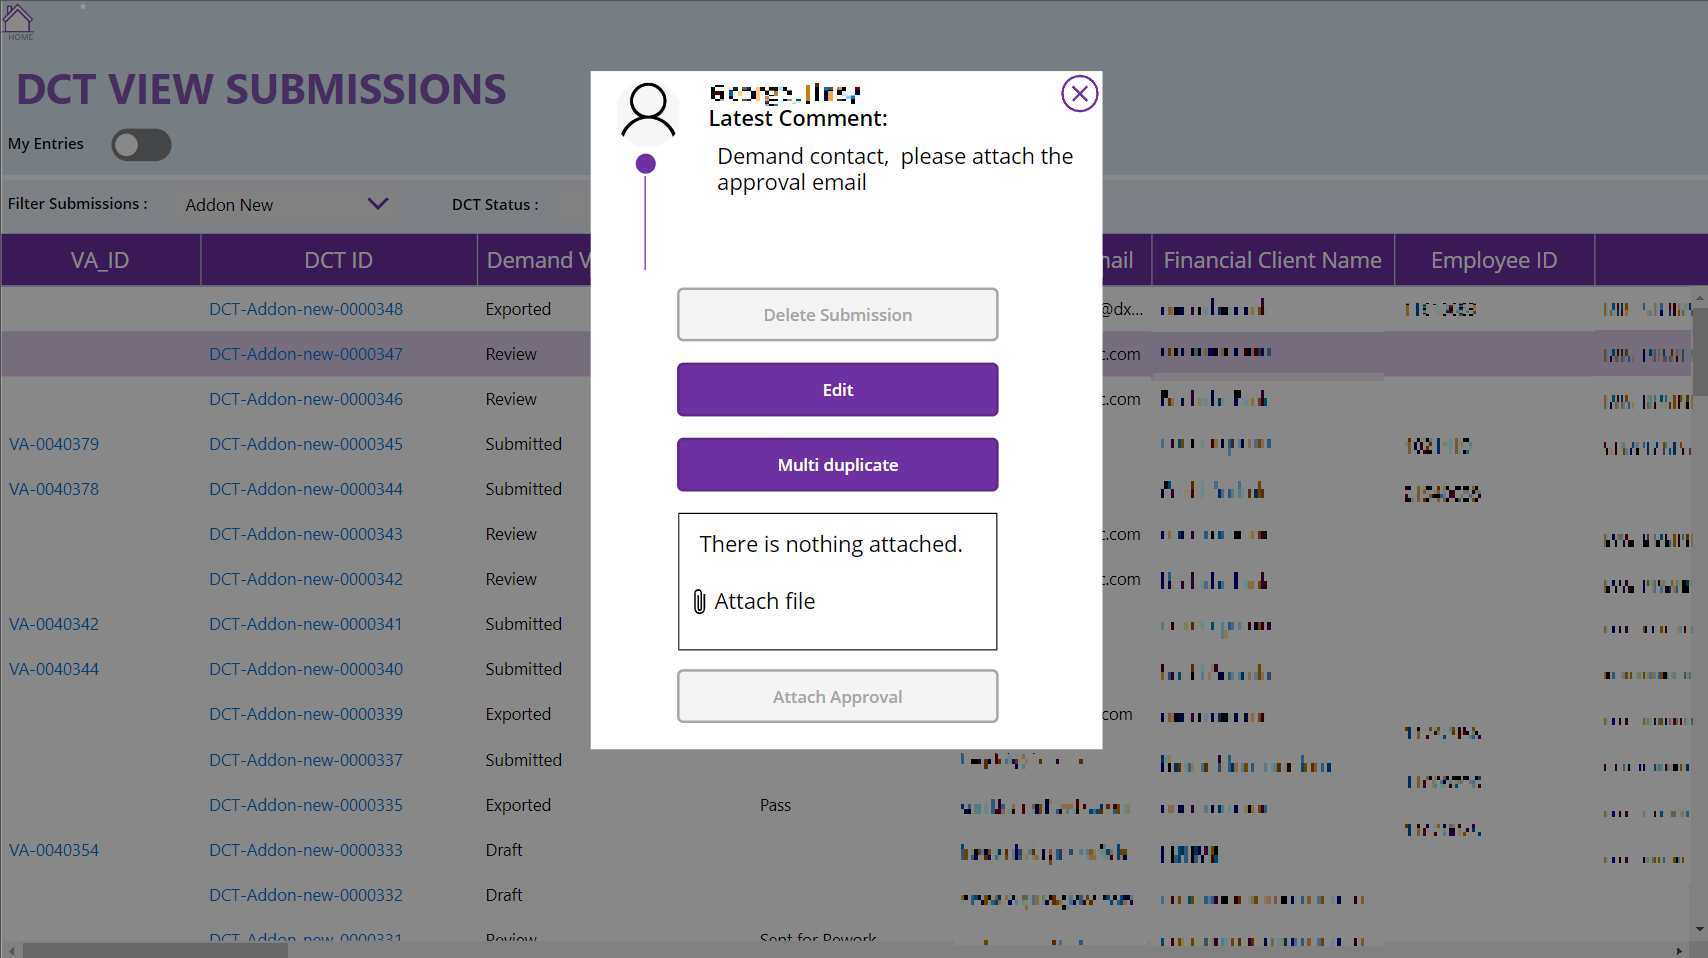
\includegraphics[scale=0.4,keepaspectratio]{Rapport de stage PFE chez DXC/figures/DCT_view_submission.png}
    \caption{DCT Position Level Management - Consultation des soumissions}
\end{figure}

Dans ce dernier nous avont les differents information saisit par l'utilisateur. en cliquant sur l'entrée un menu apparait qui contient quelque bouton, le premier permet de supprimé une entré en cas d'erreur, le deuxiem edit est utilisé pour modifier l'entrée pour corrigé une erreur, il y'a aussi l'option du multi duplicate cette derniere permet a l'utilisateur de dupliquer une entrée en plusieurs si il veut par exemple modifier que quelque information pour chaque entrée et finalement la possibiliter d'attacher un agrément exceptionnel si ce dernier est demander par les personnes qui inspecte l'entrée, d'ailleur en peut voir en haut un commentaire demander a ce dernier d'ajouter le fichier d'agréement.

\subsection{DCT Position Level Management - Validation des entrée}

\begin{figure}[H]
    \centering
    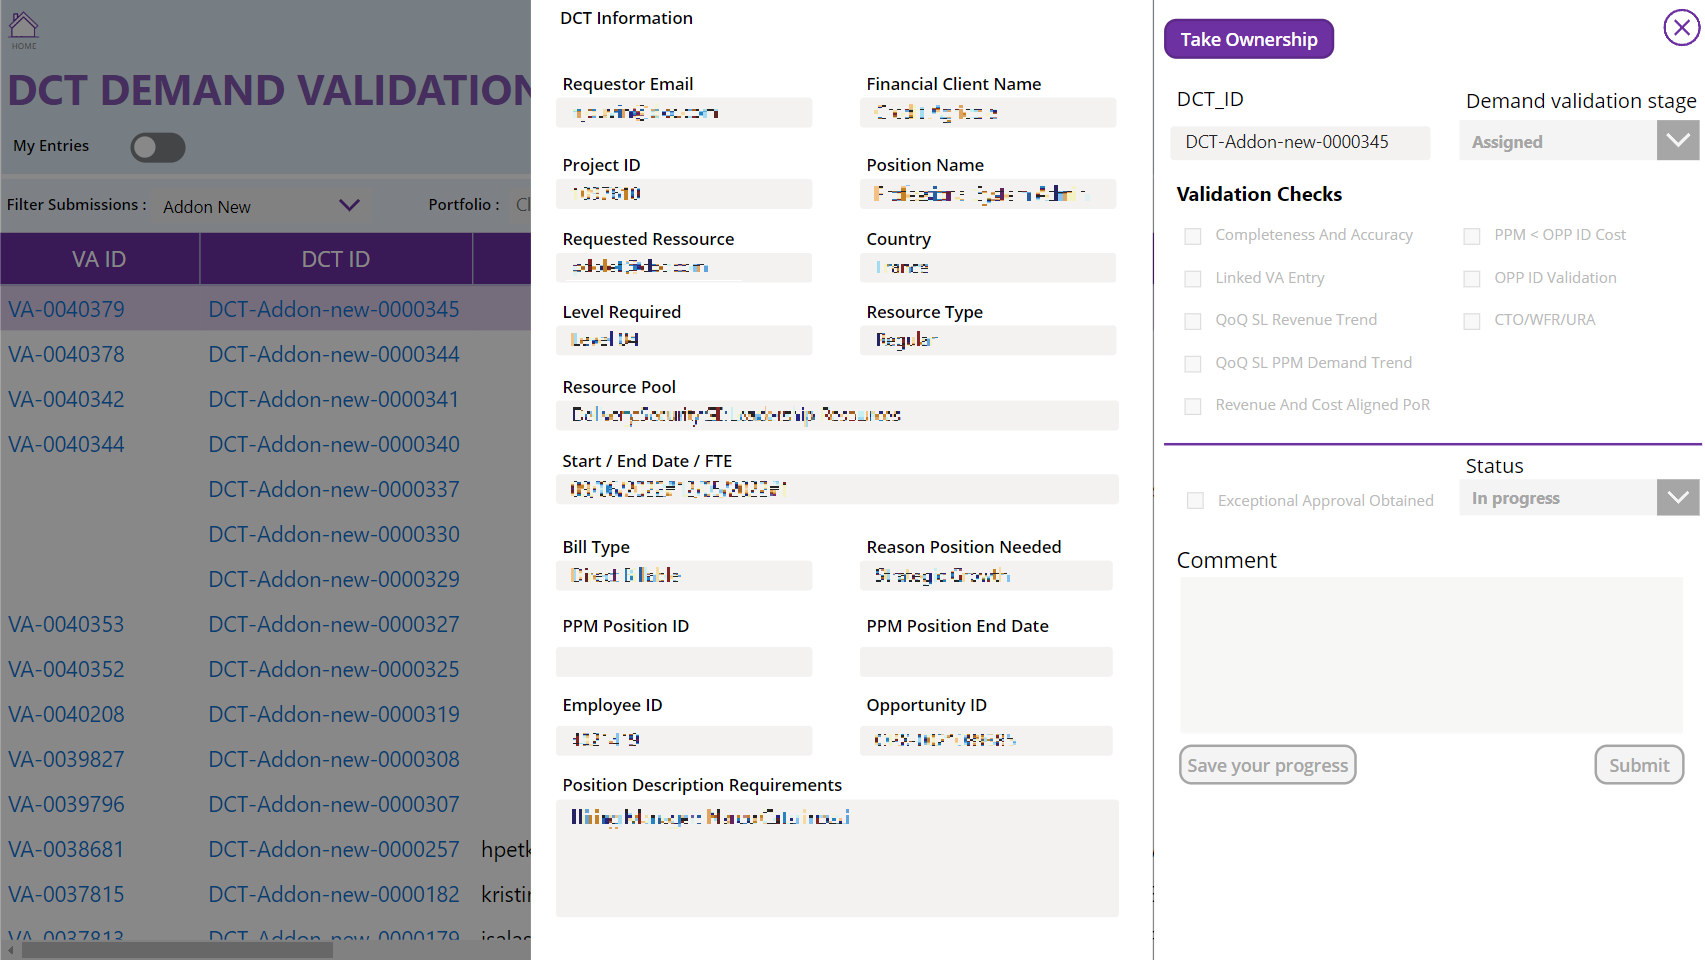
\includegraphics[scale=0.4,keepaspectratio]{Rapport de stage PFE chez DXC/figures/DCT_demand_validation_checks.png}
    \caption{DCT Position Level Management - Validation des entrée}
\end{figure}